\subsection{Overview}

\begin{figure}[ht]
  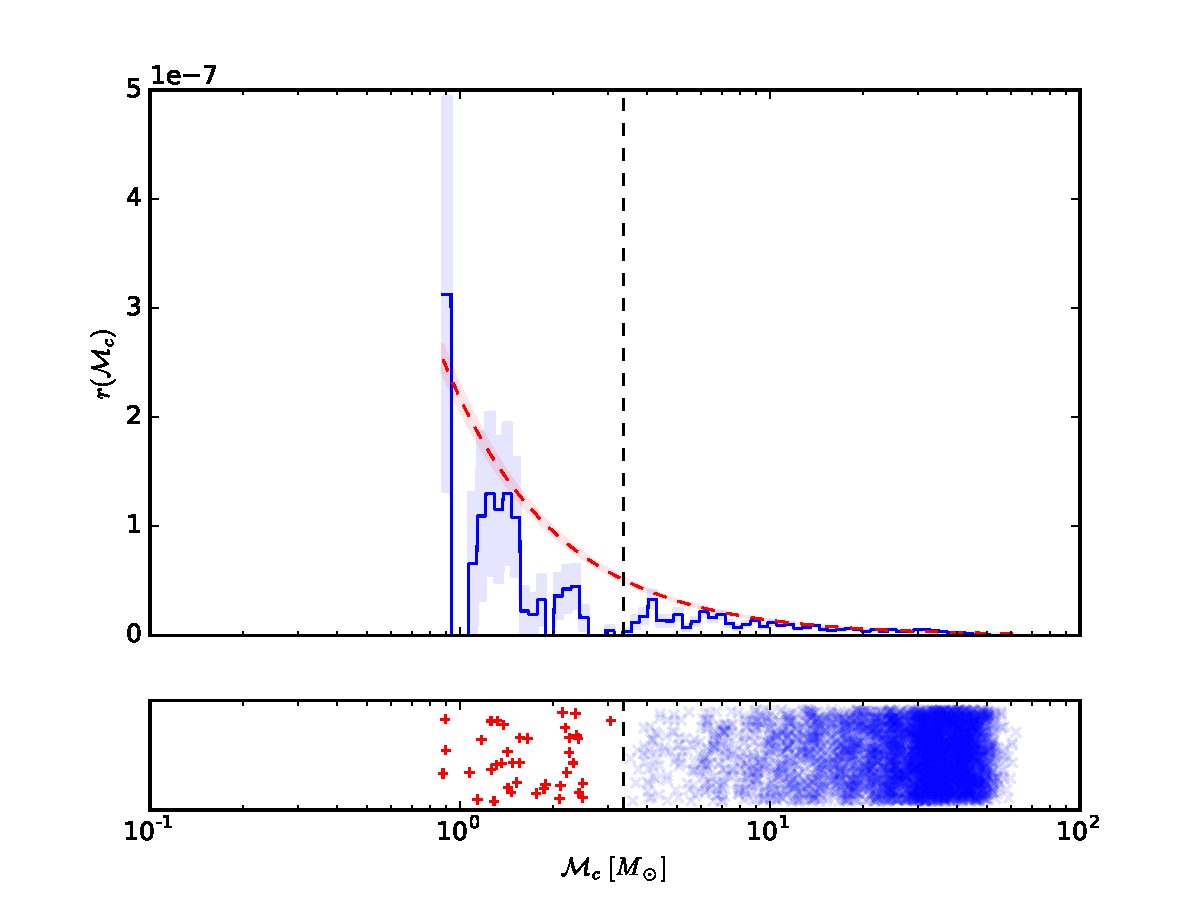
\includegraphics[width=\columnwidth]{img/chirp-mass-distribution}
  \caption{Estimated rate of compact binary mergers, based on 5000 synthetic observations. Blue line is weighted histogram fit. Red curve is power law fit. Shaded regions are 1-$\sigma$ error bars. Vertical dashed line is boundary between events with counterparts and without.}
  \label{fig:chirp}
\end{figure}

\begin{figure}[ht]
  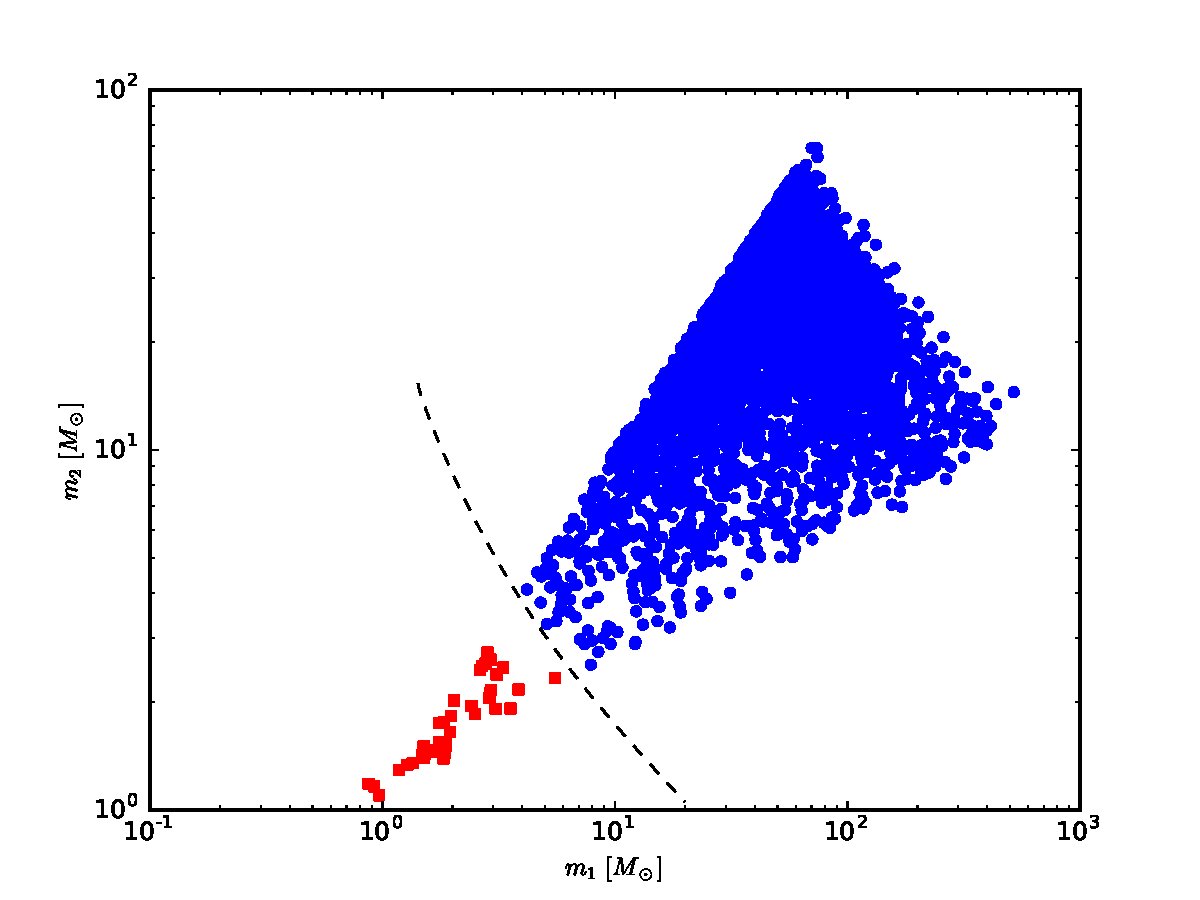
\includegraphics[width=\columnwidth]{img/output/mass-distribution}
  \caption{}
  \label{fig:2D}
\end{figure}

\begin{figure}[ht]
  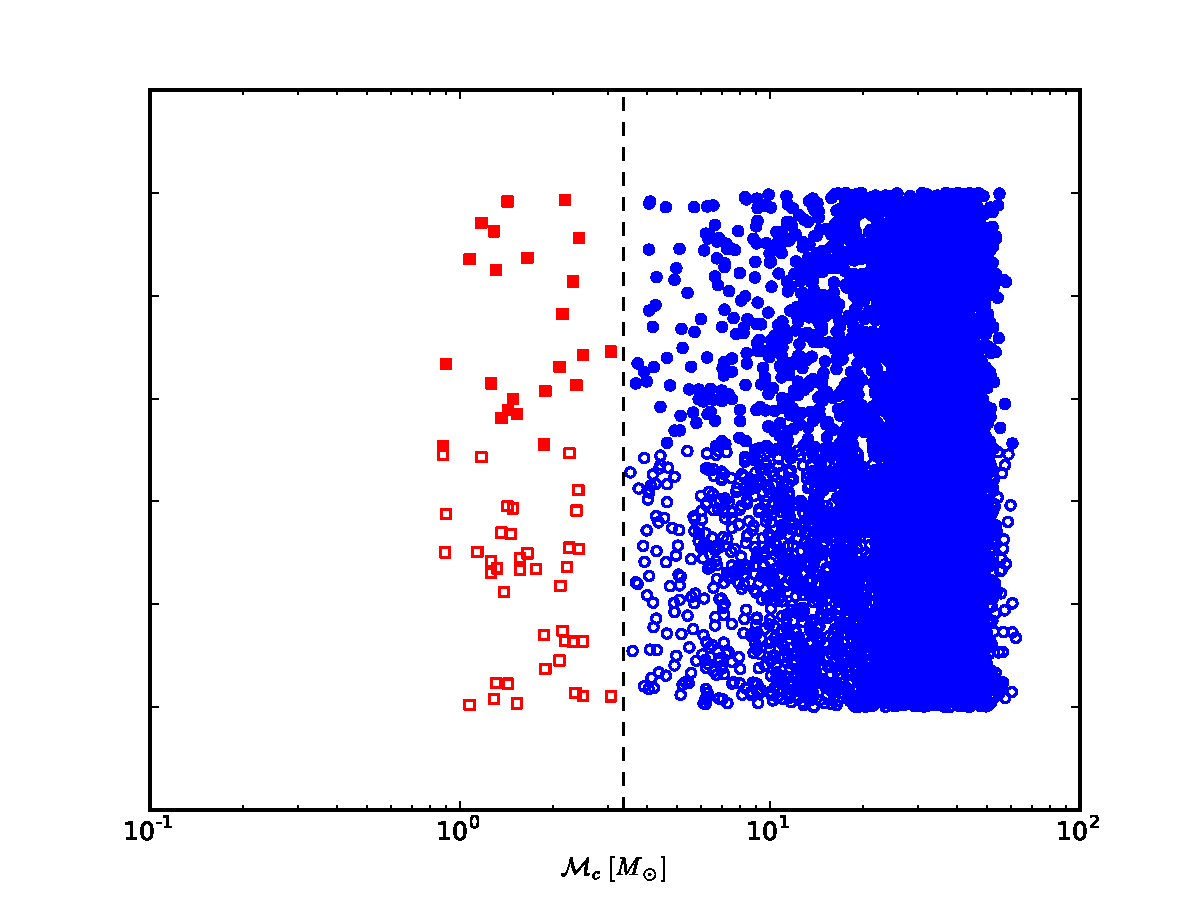
\includegraphics[width=\columnwidth]{img/output/classifier_comparison}
  \caption{This shows a selected set of the data. The red points represent the events with electromagnetic counterparts, and the blue points represent the events without electromagnetic counterparts. The filled points represent represent the train dataset, and the open points represent the rest of the data. The vertical line indicates the division between the two groups indicated by the classifier.}
  \label{fig:class}
\end{figure}

The GW observatory, the Laser Interferometer Gravitational Wave Observatory (LIGO), can provide very rapid mass estimates of candidate GW events. Since most of these detections are mostly binary black holes and electromagnetic followup is extremely expensive, only a few events can be followed up. We have therefore trained a classifier to determine if an event will have a electromagnetic followup. We trained this classifier on the first half of the data; we simply took the mid-way point betweewn the maximum chirp mass for the electromagnetic counterpart group and the nonelectromagnetic counterpart group. This can be seen in Figure \ref{fig:class}.


\subsection{Method}
The classifier was constructed simply by taking the minimum chirp mass event of the other group (no electromagnetic counterparts) and the maximum chirp mass event of the electromagnetic counterpart group and finding the mid-point between those two events. This classifier was trained from the first half of the dataset. This is visiualized by the filled points in Figure \ref{fig:class}.

\begin{table}[ht]
\caption{Chirp masses of the maximum event from the electromagnetic counterpart group, the minimum event from nonelectromagnetic counterpart group, and the vertical dividing line.}
\centering
\begin{tabular}{c c c}

\hline\hline
3.545980 & 3.065123 & 3.378711\\
\hline\hline
\end{tabular}
\label{tab:mass}
\end{table}

\subsection{Results}
The classifier correctly classified the two groups without any contamination. More importantly, this was also the case when classifying the full data set. As you can see in Figure \ref{fig:class}, the classifier correctly classified the two groups without any contamination. In the Table \ref{tab:mass}, you can see numerically that the classifier worked completely. Listed are the chirp mass for the maximum electromagnetic counterpart event and the minimum of the other group along with the chirp mass of the line that divides the group. The classifier shows a clear distinction between the two groups.



Figure \ref{fig:chirp} shows the rate vs the chirp mass with the dividing line from the classifier overplotted. This correlates to the two hump structure in the graph that represents the two groups (electromagnetic counterparts and nonelectromagnetic counterparts). Figure \ref{fig:2D} shows a similar correlation; the dividing clearly separates the two groups in  m$_{1}$-m$_{2}$ parameter space.